% Chapter 1

\chapter{Introduction} % Main chapter title

\label{Chapter1} % For referencing the chapter elsewhere, use \ref{Chapter1} 

%----------------------------------------------------------------------------------------

% Define some commands to keep the formatting separated from the content 
\newcommand{\keyword}[1]{\textbf{#1}}
\newcommand{\tabhead}[1]{\textbf{#1}}
\newcommand{\code}[1]{\texttt{#1}}
\newcommand{\file}[1]{\texttt{\bfseries#1}}
\newcommand{\option}[1]{\texttt{\itshape#1}}
%---- Summary to introduce ---
\indent\indent Historically the hallmark of biology has been the study of the individual molecular components that make up living organisms. However, since the advance of sequencing technology and high performance computing this paradigm has shifted to a more complete approach in which a biologist considers the biological networks that make up the systems that regulate and sustain life for an organism.  Continued research into genomes, gene expression and regulation continues to develop and with it so does our understanding of how each of the elements of an organism interact with one another.  \\
% * <jpbrooks@vcu.edu> 2016-08-31T02:02:42.715Z:
%
% high performance computing biology?
%
% ^ <norrissw@vcu.edu> 2016-09-01T01:45:20.361Z.
\indent Along with this systematic, holistic approach to understanding biological complexity and an increase in computational power have lead to the emergence of new methods for modeling these networks.  By using mathematics one can now represent a metabolic pathway and simulate dynamic and complex biological cellular behaviors. The ability to experimentally obtain genomic data coupled with these modeling approaches has lead to a top-down approach in which the experimental data can be integrated with the models.  This lends greater credibility in the models themselves and the ability to more accurately represent life \textit{in silico}.\\
\indent The ability to represent an organism \textit{in silico} has allowed research to be conducted without the overhead costs associated with a traditional experiment. Using computers you can now predict the outcomes of gene knockouts, and gene up/down regulation. You can also identify drug targets and study complex pathways to identify methods to turn them on, off or bypass them completely.  All of this together has lead to a deepening of our understanding of biology and increased the effectiveness of traditional experiments while reducing costs.\\
\indent However put into the time line of biological research using \textit{in silico} modeling is still very new and was initially cost prohibitive.  It takes a lot of computational overhead to be able to perform these types of experiments.  First, it requires databases that contain experimentally obtained information. Databases hosted by NCBI and other resources are freely available and often can be accessed without downloading the entire dataset. While other databases are proprietary and require you to download them before using them.  Next, the sheer amount of data generated by sequencing, genome annotation, and modeling does require a lot of physical disk space. Most of the intermediate files can be compressed or removed after a functional model is produced but even this can require gigabytes of space per model.  Finally, computational time, as in the actual cost of CPU usage while the modeling procedures are running can also be quite high but due to parallelization and job queuing engines like Sun GridEngine utilizing large amounts of computational time for generating \textit{in silico} has become much easier.\\
% * <jpbrooks@vcu.edu> 2016-08-31T02:04:04.939Z:
%
% > However put
%
% ?
%
% ^ <norrissw@vcu.edu> 2016-09-01T02:14:58.855Z.
\indent The major contributions from our work here is the ability to start from the nucleotide sequence and use our pipeline in a semi-automated fashion to reconstruct the metabolic networks of a given organism.  Previously this process was laborious and there were no tools to parse a genome annotation and derive its reactions based on the gene products determined during the annotation.  Further, we completely redesigned the MetModel into a software tool that will execute all of the necessary steps to create a constraint-based model using flux balance analysis (FBA) all the way to generate the KGML pathway maps from a single execution of the new tool.\\ 
% * <jpbrooks@vcu.edu> 2016-08-31T02:05:56.126Z:
%
% Buy there are tools, like SEED.  Probably cite SEED here and describe its limitations.
%
% Buy there are tools, like SEED.  Probably cite SEED here and describe its limitations.
%
% ^.
%--- A little bit about questions you can ask/answer in silico ---
%--- This is what it requires to do this... databases...storage...computation... etc.
%-------------------------------------------------------------------
%-----------Those Damn Databases-------- Could add details about specific database.
%--- Kegg: Used to be free, no transport reactions, no compartments
%--- SEED: Developed with funding from DOE
%--- Palsson: 
%--- Niti:
\section{Reference Databases}

\indent\indent Most \textit{in silico} tools and projects involve using a reference database at some point. The internet is a great method for sharing information from databases and a number of biological databases already exist to share information about genes, metabolites, and their reaction pathways \citep{keseler_ecocyc:_2013}.\\
\indent However, there is no standardization among these databases and often minimal curation of the data once it has been made available. So not only is there no one source of information that houses all of the data but there is also no standardized form for the information in these databases. This is particularly true when it comes to the metabolic reactions and their metabolites. This makes it difficult to verify the data in these reference databases and it also makes it difficult to obtain a consensus of information from these databases as comparing them is often difficult. \\
\indent Kyoto Encyclopedia of Genes and Genomes (KEGG), is one such database that contains genes, metabolites, reactions, and more for many different organisms\citep{ogata_kegg:_1999}. However, it lacks transport reactions and does not denote where reactions are occurring, i.e. within the cytosol, extracellular or other places.  KEGG is also no longer freely downloadable.  They still have a web page and REST API to access their data, but the user is not informed if they actively update this information or if it lags behind the paid subscribers version. The Model SEED database is another resource for genomes, metabolites, reactions and even full models\citep{overbeek_seed:_2004}. The Model SEED utilizes Rapid Annotation using Subsystems Technology (RAST) which performs the gene annotation and FBA modeling for you. RAST models can utilize genomes uploaded in FASTA or publicly available sequences in the Model SEED database.  The big limitation to using Model SEED is that this data does not appear to be actively curated at this time and thus the possibility of inaccurate or incomplete data exists. When using RAST with Model SEED, another limitation is that during the gap filling step it adds a large number of low-confidence reactions in order to complete pathways. Finally, two manually created databases were created and curated by Dr. Niti Vanee and published by Dr. Bernhard Palsson \citep{vanee_high_2013, shlomi_network-based_2008}. These databases were built to address the missing transport reactions, lack of detail about reaction locations, and otherwise update and curate the missing pieces of data for KEGG and SEED.\\
% * <jpbrooks@vcu.edu> 2016-08-31T02:09:37.236Z:
%
% > perform the modeling for you
%
% This doesn't seem like a drawback.  One of the main limitations of the SEED framework is that it adds too many low-confidence reactions to fill gaps by default.
%
% ^ <norrissw@vcu.edu> 2016-09-01T02:32:00.161Z.
% * <jpbrooks@vcu.edu> 2016-08-31T02:09:02.862Z:
%
% > reated databases
%
% reaction databases
%
% ^ <norrissw@vcu.edu> 2016-09-01T02:23:43.023Z.

%--------CBM----------
\section{Constraint-based Modeling}

\indent\indent Constraint-based modeling is an approach that has been evolving since the 1980s \citep{fell_fat_1986,majewski_simple_1990}. Initially, the approach was first shown to be viable when experimentally obtained metabolic fluxes and growth rates were shown to be consistent with computationally derived fluxes calculated from cellular objective functions \citep{savinell_optimal_1992,schuster_elementary_1994}.  Then in the early 2000s when the ability to sequence whole genomes became more readily accomplished it became possible to link the genome directly to a constraint-based model. This link paved the way for using these models to predict experimental outcomes. For example, gene knockouts and changes in cellular behavior. As biology entered into the age of 'omic data it became possible to incorporate experimentally obtained transcriptomic, exomic, proteomic, and even metabolomic data into these models to further the ability to analyze and experiment \textit{in silico}.\\
% * <jpbrooks@vcu.edu> 2016-08-31T02:11:49.956Z:
%
% > 'omic
%
% Write 'omic instead of 'omic'
%
% ^ <norrissw@vcu.edu> 2016-09-01T02:17:23.892Z.
\indent In general, constraint-based modeling works under the law of conservation of mass and that biomass growth and energy use can be used to predict metabolic fluxes for an organism \citep{schilling_theory_2000,schuster_elementary_1994}. This is accomplished by first curating all the metabolites and reactions determined, or predicted, to be present in an organism. In the case of genome-scale metabolic networks, this is done by creating a stoichiometric matrix. The stoichiometric matrix is a versatile and consistent format present in constraint-based models that indicate the number of molecules used and created in reaction. Here we focus on constraint-based modeling for genome-scale metabolic reconstructions, it has also been used for signaling, transcriptional regulation and macromolecule synthesis \citep{papin_jak-stat_2004,li_identification_2009}.\\
% * <jpbrooks@vcu.edu> 2016-08-31T02:13:08.825Z:
%
% that indicates the number of molecules used and created in each reaction
%
% ^ <norrissw@vcu.edu> 2016-09-01T02:33:26.167Z.
% * <jpbrooks@vcu.edu> 2016-08-31T02:12:34.013Z:
%
% > representing
%
% curating
%
% ^ <norrissw@vcu.edu> 2016-09-01T02:33:29.574Z.
\indent Compared to other modeling methods constraint-based modeling, in general, allows greater influence of metabolic networks for an organism and in a more realistic fashion.  More specifically, an organism \textit{in vivo} is subjected to physical, environmental, and physiochemical inhibitors and thus doesn't have an unlimited growth potential.  By having the ability to apply these constraints makes the \textit{in silico} models more accurate and also expands the ability to perform \textit{in silico} experiments. Utilizing constraint-based modeling we are able to better determine the cellular behaviors of an organism when subjected to different external or internal influences. The end result of this is a series of reaction pathways represented as a flow chart or map that represents what an organism uses to sustain life and these pathways can often vary based on the specific constraints applied to the model. 
% * <jpbrooks@vcu.edu> 2016-08-31T02:14:38.509Z:
%
% >  By considering various constraints allows us to better determine t
%
% reword
%
% ^ <norrissw@vcu.edu> 2016-09-01T02:34:17.508Z.
%------------FBA----------------
\subsection{Flux Balance Analysis}

\indent\indent Flux Balance Analysis (FBA) is one such mathematical approach to modeling and analyzing the networks that make up an organism and is particularly common in genome-scale metabolic network reconstructions \citep{schuster_elementary_1994,varma_stoichiometric_1994,thiele_genome-scale_2009}. FBA is a specific application of linear programming (LP) used to calculate and optimize the flow of metabolites over time through the biochemical reactions present in an organism to determine the steady-state flux distribution that maximizes the biomass yield. Given the stoichiometric matrix (S) and fluxes (v), the steady-state is represented as $Sv = 0$ and defines a system of linear equations. Next, to solve these equations we define an objective function, like biomass, and to predict the maximum growth rate we use $Z =c^Tv$, where c is a vector of zeros with a value of 1 only in the reaction of interest. When we're using the biomass reaction, c has a value of one so we can represent this as:\begin{center} $ Z = v\textsubscript{biomass}$\end{center}
with parameters:
\begin{center} 
$Sv + b^{src} - b^{esc} = 0$

$L \leq v \leq U$

$L^{src} \leq b^{src} \leq U^{src}$

$L^{esc} \leq b^{esc} \leq U^{esc}$
\end{center}
where $L$ and $U$ define the lower and upper bounds for each reaction, and $b^{src}$, $b^{esc}$ are the escape and source reactions specifically\citep{brooks_gap_2012}. Finally we calculate the flux values that maximize $Z$.\\

%-------------------MILP--------------
\subsection{Mixed Integer Linear Programming (MILP)}

\indent\indent Mixed Integer Linear Programming (MILP) is another modeling method.  MILP and LP are both general optimization modeling frameworks and have many applications outside of metabolic reconstructions. In comparing MILP  and LP, MILP is designed to better incorporate and optimize the use of experimentally obtained data into the model as it lets you add integer restrictions variable values\citep{bordbar_constraint-based_2014}. This step helps improve model quality by attempting to reduce false positive and false negative values from experimental data\citep{vanee_high_2013}. A false positive is when a metabolite is predicted to be present but the reaction/gene is associated with producing the metabolite is not actually shown to be present based on experimental evidence. Similarly, a false negative is when a gene or reaction is incorrectly omitted from a model but experimental evidence shows that the associated gene and gene product are in fact present. These false values are believed to be caused by post-transcriptional regulation or alternative flux distributions, which are likely from isozymes and alternative pathways.  In MetModel and Model SEED, MILP is used in FBA-Gap and GapFill which are two different algorithms designed to identify and correct reactions missing from pathways. As mentioned previously MILP can be an effective way to incorporate proteomic and other data into the pathway reconstructions \citep{shlomi_network-based_2008}.\\
% * <jpbrooks@vcu.edu> 2016-08-31T02:16:22.014Z:
%
% >  In short, the MILP algorithm is similar to FBA 
%
% No, delete this sentence.  FBA instances are linear programs (LPs).  My gap-filling models and Shlomi et al's models for reconciling experimental data are examples of MILPs.  LP and MILP are general optimization modeling frameworks.  The only difference is that MILP allows you to add integer restrictions on your variable values.
%
% ^ <norrissw@vcu.edu> 2016-09-01T01:05:48.197Z.
\indent  In the case of MILP we have a problem expressed as: 
% * <jpbrooks@vcu.edu> 2016-08-31T02:19:11.301Z:
%
% > MILP and FBA both calculate fluxes by linear programming. 
%
% No.
%
% ^ <norrissw@vcu.edu> 2016-09-01T01:05:49.821Z.
\begin{center} $maximize \hspace{0.5cm} cx + dy$ \end{center}
with parameters:
\begin{center}
$Ax+By \leq b$

$x \in \mathbb{R}_{+}^n$

$y \in \mathbb{Z}_{+}^p$\end{center}
where $cx + dy$ is the objective function, $Ax+By \leq b$ are constraints, x and y are vectors of the decision variables\citep{brooks_solving_2005}.  We can now determine solutions for our objective function if they exist. It is possible for no solution or multiple solutions to exist, and the solution that provides the best objective function value is called the optimal solution.  When we model using this type of function we look for these optimal solutions if they exist.\\


%------------------FVA----------------

\section{\textit{In Silico} Bacteria Research}

\indent\indent Modeling unicellular organisms \textit{in silico} provides a number of benefits. It allows us to work and analyze with extremophiles and pathogens without expensive equipment or health hazards. It allows us to make predictions about the outcomes for in vivo or in vitro experiments before having to incur the temporal and fiscal costs associated with performing one \citep{langowski_computer_2002}. All of this together allows us to push research of treating and preventing diseases further by focusing and developing our understanding of virulence, pathogenesis and identifying new drug targets\citep{shlomi_network-based_2008}\citep{nurputra_paramyotonia_2012}. In industry different strains or even customized genomes can be tested using these methods and we can select a particular genome or strain of bacteria that provides optimal amounts of a given metabolite which can be collected for purposes like biofuels \citep{nogales_silico_2012}. \\
%-----------ASGARD------------
\subsection{Genome Annotation using ASGARD}

\indent\indent Understanding the genes, their products and the metabolic reactions of \textit{G. vaginalis} is crucial for researching the virulence, transmission, and therapeutics.  We used the genomes of \textit{G. vaginalis} strains obtained from NCBI and other sources, then use the Automated System for Gene Annotation and Metabolic Pathway Reconstruction Using General Sequence Databases (ASGARD) to determine open reading frames and annotate the genome\citep{alves_automated_2007}. \\
\indent ASGARD can take assembled sequences in FASTA file format and perform gene annotation and predicted metabolic pathways. The data provided by ASGARD can be regarded as a draft model, and this creates the first step to a high-quality metabolic model of our organism. \\
\indent ASGARD creates these models by first determining the open reading frames within a genome by comparing it to annotated genomes stored in databases like NCBI Nucleotide and KEGG.  Once the genes and their functions are determined it places them within the appropriate pathways. From here the model can be regarded as a "rough draft" as ASGARD has made an educated guess about the pathways and enzymes present based on translated nucleotide sequence homology only. \\
\indent Using ASGARD thus allows one to take assembled genomic nucleotide sequences in FASTA file format and obtain gene annotation and predicted metabolic pathways. The data provided by ASGARD begins the search for an accurate metabolic model of our organism. We used both well-documented strains (i.e. strains that have already been annotated thoroughly) and novel strains. This "draft" model was then integrated with our MetModel where a series of scripts were used to integrate gene expression data, metabolic data and our other information to increase the accuracy and precision of the draft model.\\

%--------MetModel----------
\subsection{Metabolic Pathway Reconstruction Using MetModel}

\indent\indent For our purposes, ASGARD is just the first step and the model will undergo further revisions as it goes through the MetModel pipeline.  The MetModel pipeline will gap fill pathways then use FBA to derive the reactions rates for optimal growth. It can then be used to build KGML maps of the reaction pathways and if available increase the accuracy and confidence we have in the metabolic reconstruction model by incorporating experimental data. mRNA expression data can be obtained from NCBI Gene Expression Omnibus (GEO) and incorporated during this process in order to provide experimental data to support the analysis and solutions obtained from the FBA. 
% * <jpbrooks@vcu.edu> 2016-08-31T02:23:11.906Z:
%
% > etModel pipeline will use FBA (Flux Balance Analysis) to increase the accuracy and confidence we have in the model.
%
% No.
%
% ^ <jpbrooks@vcu.edu> 2016-08-31T02:24:06.745Z:
%
% Again, what is "the model?"  FBA gives us reaction rates for optimal growth.
%
% ^ <norrissw@vcu.edu> 2016-09-01T11:56:51.079Z.
% * <jpbrooks@vcu.edu> 2016-08-31T02:22:08.577Z:
%
% > the model
%
% It is unclear what you mean by "the model."
%
% ^ <norrissw@vcu.edu> 2016-09-01T11:56:49.617Z.
\indent Finally the model pathways were viewed and reviewed manually using KGML-ED\citep{klukas_dynamic_2007}. \\
\indent MetModel is Python library which can be used in a pipeline to gap-fill reaction pathways determined by ASGARD to then apply a constraint-based modeling approach.  This modeling approach considers all of the potential biochemical reactions and then applies constraints in the same way that an organisms environment, physiochemical, regulatory and evolutionary sources would constrain its growth potential. Thus MetModel allows us to incorporate metabolic data with gene/reaction network, thermodynamics, gene regulation and other information. Using MetModel allows us to consider the states that an organism can and cannot achieve which gives us a broader view as to the factors that are involved in determining an organism's survivability, growth potential and even its ability to produce metabolites under various conditions and with greater accuracy than other modeling tools\citep{roberts_proteomic_2009}. \\
% * <jpbrooks@vcu.edu> 2016-08-31T02:25:26.023Z:
%
% > sing the FBA approach, MetModel
%
% It's not clear what the difference between MetModel and FBA is.
%
% ^ <norrissw@vcu.edu> 2016-09-01T02:39:14.531Z.
% * <jpbrooks@vcu.edu> 2016-08-31T02:24:31.507Z:
%
% >  MetModel is Python library
%
% Maybe cite Seth's T. cruzi paper here.
%
% Maybe cite Seth's T. cruzi paper here.
%
% ^ <norrissw@vcu.edu> 2016-09-01T02:40:40.032Z.
\indent In order for MetModel to perform these tasks it first converts the biochemical reaction network reconstruction into a mathematical form.  To do this we went through three steps, the first is the analysis of the reactions within the network. They usually fall into three main categories like metabolic, regulatory, and signaling. Next, the data derived from this analysis is used to form the stoichiometric matrix. This stoichiometric matrix is the mathematical representation or map where the chemical constraints are applied to the model. Now that we had our mathematical representation of the organism's pathways, flux balance analysis (FBA) can be performed to generate a solution or solutions\citep{orth_what_2010}. FBA calculates the flow of metabolites through the network, and this makes it possible to predict the production rates of metabolites, the growth rate of an organism, and analyze specific pathways and even predict experimental outcomes \citep{lee_complementary_2005}. Put another way these \textit{in silico} models allow predictions of  phenotypes given a set of genes and reactions. For example, we can perform an \textit{in silico} knockout model or we can try to optimize gene products which is particularly useful for nitrogen-fixing bacteria used in biofuel production \citep{nogales_silico_2012}. In the case of pathogens like \textit{G. vaginalis} we can use MetModel to test out new drug designs, or better understand how it might infect and gain a foothold among the normal vaginal bacterial community.\\
\indent Using this modeling approach considers all of the potential biochemical reactions and then applies constraints in the same way that an organism's environment, physiochemical, regulatory and evolutionary sources would constrain its growth potential. Thus MetModel allows us to incorporate metabolic data with gene/reaction network, thermodynamics, gene regulation and other constraints. This approach to modeling allows us to consider the states that an organism can and cannot achieve which gives us a broader view as to the factors that are involved in determining an organism's survivability, growth potential and even its ability to produce metabolites under various conditions.

%----------------------------------------------------------------------------------------Gardnerella--------
\section{Gardnerella}

\indent\indent \textit{Gardnerella} is a genus of bacteria for which \textit{G. vaginalis} is presently the only known species. \textit{G. vaginalis} is a clinically significant bacterium that can disrupt the normal vaginal flora and cause bacterial vaginosis (BV). BV is a major medical problem, causing discomfort to millions of women every year and has been shown to cause complications for many pregnant women resulting in preterm labor and birth which may result in death or long-term health problems for the baby. Many patients with BV are asymptomatic but occasionally have yellow or gray discharge, irritation, or a foul odor. Diagnosing BV can be difficult especially if the patient is asymptomatic. Figure ~\ref{fig:ClueCells} shows a diagrammatic depiction of how these bacterial cells are identified once stained. \textit{G. vaginalis} is not considered to be the single microbe inducing BV but rather a signal that the normal vaginal tract flora has been disrupted, thus paving the way for other anaerobes to work synergistically to reduce the protective, hydrogen peroxide producing {\it Lactobacillus} species that suppress the harmful bacteria from proliferating. Further, the \textit{G. vaginalis} cells are so small they do not reliably show up as gram-positive and thus can be difficult to detect. Presently, the main treatment for patients with BV caused by \textit{G. vaginalis} are antibiotics such as clindamycin or metronidazole.\\
\begin{figure}[h]
\centering
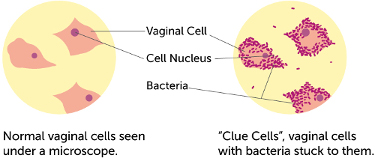
\includegraphics{Figures/ClueCells}
\decoRule
\caption[Clue Cells]{Artist's rendering of how a clinician is able to use microscopy to identify \textit{G. vaginalis} cells that have infected vaginal tissue. Image reprinted with permission from: \citep{_bacterial_????} }
\label{fig:ClueCells}
\end{figure}
\indent\textit{Gardnerella vaginalis} is a gram-variable anaerobic coccobacilli. It is a facultative anaerobe and can metabolize glucose under both aerobic and anaerobic conditions, and has a complex metabolism \citep{patterson_analysis_2010}. It is the sole member of the \textit{Gardnerella} genus and is a small (\(1.0  \mu m\)), non-motile and nonspore-forming bacterium. The \textit{G. vaginalis} genome is a circular DNA and is without plasmids. Within \textit{G. vaginalis} there are genetic variants that include both virulent and avirulent strains. It is considered to be a key component in the initiation and progression of BV \citep{schwebke_role_2014}. Models of the pathogenesis of BV suggest the virulent stains of \textit{G. vaginalis} are usually transmitted through sexual intercourse and its virulence factors allow it to adhere to vaginal epithelial tissue.  Once attached to epithelial cells it creates a biofilm where a community of normally dormant vaginal anaerobes flourish. \textit{Gardnerella vaginalis} also exhibits cytotoxic activities \citep{patterson_analysis_2010}. Once established this biofilm community then aggressively competes with microorganisms of the typical vaginal flora. For example, the predominant \textit{Lactobacillus} populations that help regulate a healthy pH, and creates conditions for an overgrowth of \textit{G. vaginalis} and its associated pathogenic anaerobes. This microfloral replacement results in the clinical symptoms associated with BV (odor, discomfort, itch etc.). Studying the pathogens' genes gives biochemical and metabolic information to interpret its cooperative and competitive interactions with its human host and co-occurring species, suggesting how it overgrows and out-competes the established healthy microflora. Understanding the etiology of the disease will hopefully give insights into the best methods to prevent and control it.   \\
\indent There are over 1,365 genes in the reference genome of \textit{Gardnerella vaginalis ATCC 14019}. Not all of the \textit{G. vaginalis} strains identified are virulent and more research is needed in order to understand the virulence factors. It does appear that \textit{G. vaginalis} forms symbiotic relationships with other vaginal anaerobes that are normally dormant, and these relationships contribute to its success, resulting in symptoms and progression of BV\citep{gardner_pathogenicity_1983,schwebke_role_2014}.